\documentclass[11pt]{amsart}
\usepackage{geometry}                % See geometry.pdf to learn the layout options. There are lots.
\geometry{letterpaper}                   % ... or a4paper or a5paper or ... 
%\geometry{landscape}                % Activate for for rotated page geometry
%\usepackage[parfill]{parskip}    % Activate to begin paragraphs with an empty line rather than an indent
\usepackage{graphicx}
\usepackage{amssymb}
\usepackage{epstopdf}
\usepackage{subfig}
\DeclareGraphicsRule{.tif}{png}{.png}{`convert #1 `dirname #1`/`basename #1 .tif`.png}
\bibliographystyle{abbrv}

\title{Evolution of information flow on the internet: Project Milestone}
\author{Kevin Leung}
%\date{}                                           % Activate to display a given date or no date

\begin{document}
\maketitle
As internet usage has grown recently, it has become important in our lives and has affected the way that we act and think. Particularly, people today consume and produce large amounts of media on the internet and in ways very different from before. A common complaint about this change, however, is that we experience an information overload, with status updates constantly coming in from social networks, such as Twitter or Facebook, in small bursts relating to minor events. Some claim that there's a cost to this continuous flow of relatively unimportant information: we no longer pay attention to the big ideas or big movements in the world because we're stuck in the minutia \cite{big-idea} \cite{egypt}. By looking at the flow of information through social bookmarks on the internet as a graph over time, we can see how valid this claim is.
\section{Related Work}
Kleinberg \cite{bursty-original} describes information streams as having bursty behavior, where individual events grow and disappear quickly . Kumar et al. \cite{bursty} applied this behavior specifically to the blogosphere. They looked at the evolution of the blogosphere into small communities and characterized its bursty behavior. Their time graph was able to also track the evolution of the network and look at when bursts happen. 

Gruhl et al. \cite{gruhl} looked specifically at how information spread through the blogosphere. By focusing on specific topics, they distinguished between the regular, long-running "chatter" around certain topics versus a "spike" from specific events. They also focus in on individuals to see how they behaved.

Leskovec et al. \cite{cascade} looked at cascades that occurred in the blogosphere. They discovered that most cascades are small, and these tended to be more wide than deep. In contrast to the last paper, however, they did not find bursty behavior across the blogosphere. Additionally, they also propose the \textit{Cascade generation model} to model the data they found.
\section{Data Collection}
For this project, I decided to use data from delicious, a social bookmarking site. Since I'm interested in the long-term evolution of behavior and long-range effects, it was important to have a dataset spanning several years, with the source of the bookmark as well as the time of the bookmark. G\"orlitz et al. \cite{goerlitz} has a corpus\footnote[1]{https://www.uni-koblenz.de/FB4/Institutes/IFI/AGStaab/Research/DataSets/PINTSExperimentsDataSets/} with about 70 million bookmarks spanning from January 2003 through December 2006. The data included the date of the bookmark, the tags associated with the bookmark (which I discarded), an identifier for the bookmark target URL, and an identifier for the user. Unfortunately, because the URL itself wasn't included, I was unable to find any further information about the webpages, such as the type (commercial, blog, etc.) or the original time of creation. Particularly, the first bookmark associated with each node is effectively treated as the creation time of that cascade, though it might be long after the webpage was created.

To compare activity over time efficiently, I split the graph into 4 segments, each corresponding to a year. Between each year, the number of bookmarks increased significantly, jumping by an order of magnitude for the first 3 years:

\vspace{10pt}

\begin{tabular}{| l | l |}
 \hline
Year & Bookmark Count \\ \hline
2003 & 106549\\ \hline
2004 & 1833989 \\ \hline
2005 & 16120787 \\ \hline
2006 & 54627807 \\ \hline
\end{tabular}

\vspace{10pt}

One consequence of splitting these bookmarks by year is that some URLs may be split across years and treated as 2 separate cascades. Since the data doesn't exist before 2003 and isn't available after 2006, this seemed like a consistent, if unfortunate, compromise to make. In the analysis below, cascades of size 1 were removed since they weren't relevant.

\section{Results}
\subsection{Summary Statistics}
The initial analysis on the data was to see if there was any difference between the years at all. Although the number of networks increased from year to year, it's also possible that the network scaled perfectly with it. First, I looked at the distribution over the bookmark counts for particular bookmark targets:

\begin{figure}
	\centering
	\subfloat[]{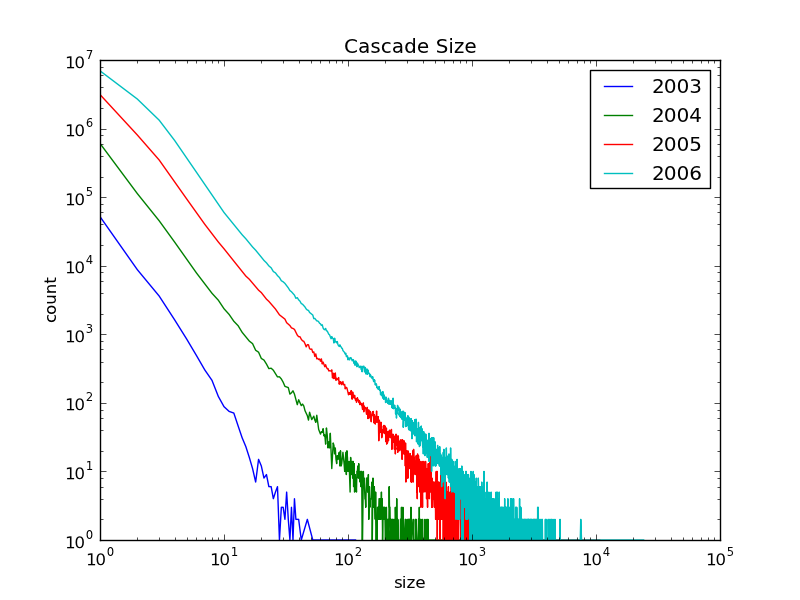
\includegraphics[width=4in]{cascade_sizes.png}}
	\subfloat[]{\begin{tabular}{| l | l | l |} \hline
		Year & Regression $\alpha$ & MLE $\alpha$ \\ \hline
		2003 & 2.75 & 5.00 \\ \hline
		2004 & 2.00 & 4.03\\ \hline
		2005 & 1.71 & 3.26\\ \hline
		2006 & 1.66 & 2.70 \\ \hline
		\end{tabular}
}
\caption{}
\end{figure}

Plotted on a log-log scale in figure 1, the cascade sizes look roughly linear, suggesting a power law distribution with the $\alpha$s in the table on the right. These results intuitively make sense: many pages will only be bookmarked once, with larger counts being less likely. Interestingly, this isn't simply a matter of scale: the $\alpha$ also appears to be decreasing from year to year, though at a slower rate. This change suggests that more bookmarks are pointing to the same page. One possible explanation for this is the delicious users have become more social over time and are tending to bookmark more things based on what other are of interest instead of finding pages more randomly.

\subsection{Time Course of Bookmarks}

Past the size of the cascades, I'm also in the time course of bookmarks and how long these cascades stretch out. To do this, I took the average time difference from the beginning of the cascade to the subsequent nodes. These were both averaged over all cascades and split by cascade size.

To compare how interesting these results were, I also generated a random network. Inspired by random rewiring on times\cite{bursty}, I randomized the times of all of the bookmarks, which should evenly distribute the time overs all of the nodes and kill the bursty behavior. This method is fairly crude, and I want to use a slightly better one that retains the starting time for the nodes. Both of these results are below in figure 2.

\begin{figure}
	\centering
	\subfloat[]{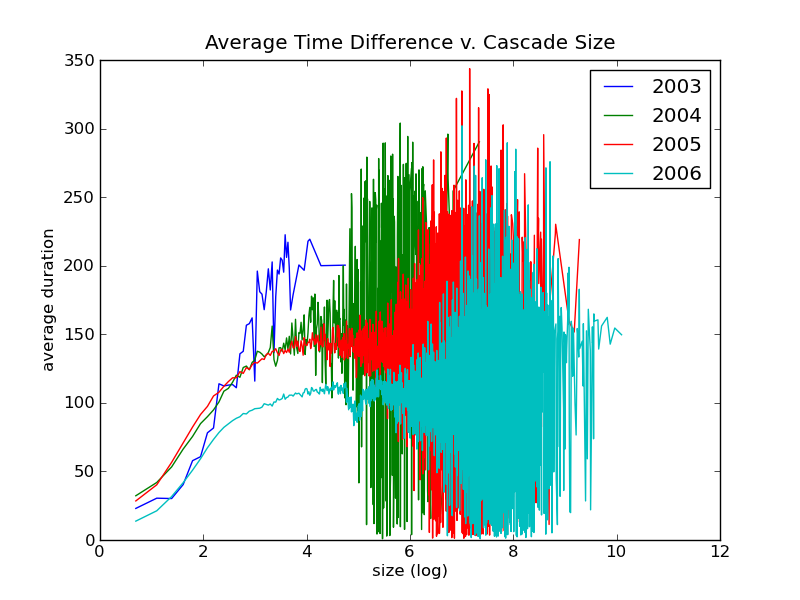
\includegraphics[width=3in]{time_plot.png}}
	\subfloat[]{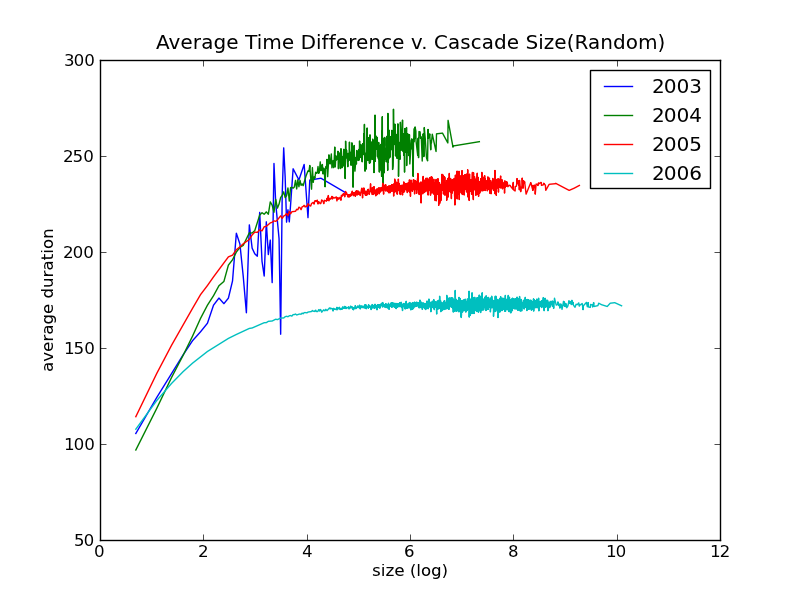
\includegraphics[width=3in]{time_plot_random.png}} \\
	\subfloat[]{\begin{tabular}{| l | l | l |} \hline
		Year & Network Average & Random Average \\ \hline
		2003 & 32.3 & 120.87\\ \hline
		2004 & 50.3 & 122.66 \\ \hline
		2005 & 50.79 & 139.58 \\ \hline
		2006 & 30.47 & 123.58 \\ \hline
		\end{tabular}
}
\caption{Sorry these are line plots instead of scatterplots. I was having difficulty with matplotlib displaying colors}
\end{figure}

Interestingly, There's a drop in the average time difference between years in both the real and random data. I immediately don't have an explanation for this result, though my intuition is that it could be related to the year-end truncation of data and the process of "filling in" the details as the network grows. Looking at the raw data, I noticed very high variance in the average time difference for various cascades of the same size. In the case of a cascade of 2, having one bookmark in January and one in December has a huge effect in pulling up the average.

A good result that we would expect is that the network average time difference is significantly lower than that of the random network average time difference. This confirms our belief that most activity tends to happen early and around the same time instead of being distributed across the year. Again, I'm certain that the average time difference of the random network lying right around 1/3 of the year is no coincidence, but I haven't done the math for it. Unfortunately, there appears to be no other pattern with this data.

In continuing work, I want to compare the results to a generative model of cascades, such as the \textit{Cascade generation model}\cite{cascade}. Presumably, there's some distribution over the likelihood of different shapes of cascades, and changes in that distribution from year to year may not be statistically significant. This model gives us a baseline for how frequently to expect uncommon events and again how that changes with the size of the graph over time.

\section{Conclusion}
After getting through cleaning the data and looking at the initial statistics, the results are promising in I found some differences to investigate. My primary concern with this particular dataset is that there actually isn't as rich of data as I had originally hoped. Without any understanding of the social structure of delicious or the nature of the webpages, there is little to work with. A major oversight I had with this is that there actually isn't significantly complex network structure: the only connection between various bookmarks is that they're bookmarking the same thing, which makes the cascades somewhat trivial.

It will be somewhat tricky to determine what differences are caused by actual fundamental shifts in behavior versus the effects from scaling a network to a much larger size, though random baseline models should attempt to distinguish that. Given these concerns, however, I believe that I will need to work on more clever analyses to draw out the characteristics I'm looking for in the data. Particularly, my analyses so far have worked around the main issue I'm looking at: how to contrast short, big memes versus long, persisting ideas. Finding the proper metric for that will be critical to the success of this project.

\bibliography{milestone}
\bibliographystyle{abbrv}

\end{document}  